\documentclass[aspectratio=169,11pt]{beamer}

% ── Packages ──────────────────────────────────────────────────────────────────
\usepackage[utf8]{inputenc}
\usepackage[T1]{fontenc}
\usepackage{lmodern}
\usepackage{amsmath,amssymb,amsthm,mathtools}
\usepackage{bm}
\usepackage{graphicx}
\usepackage{tikz}
\usetikzlibrary{arrows.meta,positioning,shapes.geometric,fit,calc,decorations.pathreplacing}
\usepackage{pgfplots}
\pgfplotsset{compat=1.18}
\usepackage{booktabs}
\usepackage{listings}
\usepackage{hyperref}
\usepackage{xcolor}
\usepackage{algorithm}
\usepackage{algpseudocode}
\usepackage{natbib}

% ── Theme: clean research style ───────────────────────────────────────────────
\usetheme{Boadilla}
\usecolortheme{default}
\usefonttheme{professionalfonts}
\setbeamertemplate{navigation symbols}{}
\setbeamertemplate{footline}[frame number]

\definecolor{mlblue}{RGB}{0,82,147}
\definecolor{mlorange}{RGB}{220,100,0}
\definecolor{mlgreen}{RGB}{0,130,70}
\definecolor{mlred}{RGB}{180,30,30}
\definecolor{mlgray}{RGB}{80,80,80}
\definecolor{mlbg}{RGB}{245,248,252}

\setbeamercolor{structure}{fg=mlblue}
\setbeamercolor{frametitle}{bg=mlblue,fg=white}
\setbeamercolor{block title}{bg=mlblue,fg=white}
\setbeamercolor{block body}{bg=mlbg}
\setbeamercolor{block title alerted}{bg=mlorange,fg=white}
\setbeamercolor{block body alerted}{bg=mlorange!10}
\setbeamercolor{block title example}{bg=mlgreen,fg=white}
\setbeamercolor{block body example}{bg=mlgreen!10}

% ── Section progress bar ──────────────────────────────────────────────────────
\setbeamertemplate{headline}{%
  \begin{beamercolorbox}[wd=\paperwidth,ht=2.25ex,dp=1ex]{section in head/foot}%
    \insertsectionnavigationhorizontal{\paperwidth}{}{}%
  \end{beamercolorbox}%
}

% ── Math macros ───────────────────────────────────────────────────────────────
\newcommand{\R}{\mathbb{R}}
\newcommand{\N}{\mathbb{N}}
\newcommand{\E}{\mathbb{E}}
\newcommand{\Prob}{\mathbb{P}}
\newcommand{\norm}[1]{\left\lVert#1\right\rVert}
\newcommand{\abs}[1]{\left|#1\right|}
\newcommand{\inner}[2]{\left\langle#1,\,#2\right\rangle}
\newcommand{\vect}[1]{\bm{#1}}
\newcommand{\mat}[1]{\mathbf{#1}}
\newcommand{\grad}{\nabla}
\DeclareMathOperator*{\argmin}{arg\,min}
\DeclareMathOperator*{\argmax}{arg\,max}
\DeclareMathOperator{\softmax}{softmax}
\DeclareMathOperator{\sigmoid}{\sigma}
\DeclareMathOperator{\Tr}{Tr}
\DeclareMathOperator{\diag}{diag}

% ── Theorem styles ────────────────────────────────────────────────────────────
\newtheorem{proposition}{Proposition}
\newtheorem{assumption}{Assumption}

% ── Code style ────────────────────────────────────────────────────────────────
\lstset{
  language=Python,
  basicstyle=\ttfamily\scriptsize,
  keywordstyle=\color{mlblue}\bfseries,
  commentstyle=\color{mlgray}\itshape,
  stringstyle=\color{mlgreen},
  numberstyle=\tiny\color{mlgray},
  numbers=left,
  numbersep=4pt,
  breaklines=true,
  frame=single,
  backgroundcolor=\color{black!4},
  showstringspaces=false,
}

% ── Title ─────────────────────────────────────────────────────────────────────
\title[Short Title]{Full Research Paper Title:\\A Subtitle If Needed}
\author[First Author et al.]{%
  First Author\inst{1} \and
  Second Author\inst{2}
}
\institute[]{%
  \inst{1} Department, University A \and
  \inst{2} Department, University B
}
\date{Conference/Workshop Name, \the\year}

% ══════════════════════════════════════════════════════════════════════════════
\begin{document}
% ══════════════════════════════════════════════════════════════════════════════

\begin{frame}
  \titlepage
\end{frame}

\begin{frame}{Outline}
  \tableofcontents
\end{frame}

% ── 1. PROBLEM ────────────────────────────────────────────────────────────────
\section{Problem Statement}

\begin{frame}{Problem Statement}
  \begin{block}{Formal Problem}
    Given $\mathcal{D} = \{(\vect{x}_i, y_i)\}_{i=1}^{N}$ with $\vect{x}_i \in \R^d$, $y_i \in \mathcal{Y}$,
    find $f_\theta : \R^d \to \mathcal{Y}$ that minimizes:
    \begin{equation}
      \mathcal{L}(\theta) = \frac{1}{N}\sum_{i=1}^{N}\ell\!\left(f_\theta(\vect{x}_i),\, y_i\right) + \lambda\,\Omega(\theta)
    \end{equation}
  \end{block}
  \vspace{0.4em}
  \textbf{Challenges:}
  \begin{enumerate}
    \item<2-> Challenge 1 (non-convexity, high dimensionality, \ldots)
    \item<3-> Challenge 2
    \item<4-> Challenge 3 $\Rightarrow$ \alert{our contribution}
  \end{enumerate}
\end{frame}

% ── 2. RELATED WORK ───────────────────────────────────────────────────────────
\section{Related Work}

\begin{frame}{Related Work}
  \begin{columns}[T]
    \begin{column}{0.48\textwidth}
      \begin{exampleblock}{Approach A \citep{smith2020}}
        \begin{itemize}
          \item Pro: strong theoretical guarantees
          \item Con: $\mathcal{O}(n^3)$ complexity
        \end{itemize}
      \end{exampleblock}
    \end{column}
    \hfill
    \begin{column}{0.48\textwidth}
      \begin{exampleblock}{Approach B \citep{jones2021}}
        \begin{itemize}
          \item Pro: scalable
          \item Con: no convergence proof
        \end{itemize}
      \end{exampleblock}
    \end{column}
  \end{columns}
  \vspace{0.6em}
  \begin{alertblock}{Gap}
    No prior work simultaneously addresses efficiency \textit{and} theoretical soundness.
  \end{alertblock}
\end{frame}

% ── 3. METHOD ─────────────────────────────────────────────────────────────────
\section{Method}

\begin{frame}{Method Overview}
  \centering
  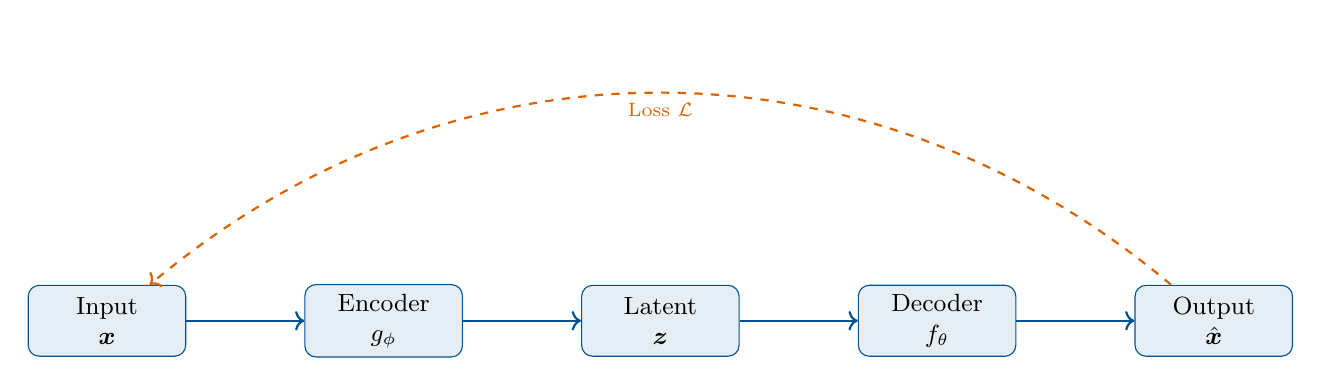
\begin{tikzpicture}[
    box/.style={rectangle,rounded corners,draw=mlblue,fill=mlblue!10,
                minimum width=2cm,minimum height=0.9cm,align=center,font=\small},
    arr/.style={->,thick,mlblue},
  ]
    \node[box] (inp) {Input\\$\vect{x}$};
    \node[box,right=1.5cm of inp] (enc) {Encoder\\$g_\phi$};
    \node[box,right=1.5cm of enc] (lat) {Latent\\$\vect{z}$};
    \node[box,right=1.5cm of lat] (dec) {Decoder\\$f_\theta$};
    \node[box,right=1.5cm of dec] (out) {Output\\$\hat{\vect{x}}$};
    \draw[arr] (inp) -- (enc);
    \draw[arr] (enc) -- (lat);
    \draw[arr] (lat) -- (dec);
    \draw[arr] (dec) -- (out);
    \draw[arr,mlorange,dashed,bend right=40]
      (out) to node[below,font=\scriptsize]{Loss $\mathcal{L}$} (inp);
  \end{tikzpicture}
\end{frame}

\begin{frame}{Theoretical Analysis}
  \begin{theorem}[Convergence]
    Under Assumptions 1--3, Algorithm~1 converges to a stationary point at rate:
    \begin{equation}
      \frac{1}{T}\sum_{t=1}^{T}\E\!\left[\norm{\grad_\theta\mathcal{L}(\theta_t)}^2\right]
      \;\leq\; \mathcal{O}\!\left(\frac{1}{\sqrt{T}}\right)
    \end{equation}
  \end{theorem}
  \vspace{0.5em}
  \textit{Proof sketch:} Use $L$-smoothness + unbiased gradient estimator + step-size $\eta_t = \mathcal{O}(1/\sqrt{t})$.
\end{frame}

% ── 4. EXPERIMENTS ────────────────────────────────────────────────────────────
\section{Experiments}

\begin{frame}{Experimental Setup}
  \begin{columns}[T]
    \begin{column}{0.48\textwidth}
      \textbf{Datasets}
      \begin{itemize}
        \item CIFAR-10 / CIFAR-100
        \item ImageNet-1K
        \item Custom benchmark
      \end{itemize}
      \textbf{Baselines}
      \begin{itemize}
        \item SGD, Adam, AdamW
        \item Method A \citep{smith2020}
        \item Method B \citep{jones2021}
      \end{itemize}
    \end{column}
    \hfill
    \begin{column}{0.48\textwidth}
      \textbf{Metrics}
      \begin{itemize}
        \item Top-1 / Top-5 accuracy
        \item Convergence speed (epochs to 90\%)
        \item Wall-clock time (hrs)
      \end{itemize}
      \textbf{Hardware}
      \begin{itemize}
        \item 8× A100 80GB GPUs
        \item PyTorch 2.0
      \end{itemize}
    \end{column}
  \end{columns}
\end{frame}

\begin{frame}{Main Results}
  \begin{table}
    \centering
    \caption{Top-1 accuracy (\%) on ImageNet. Best in \textbf{bold}.}
    \small
    \begin{tabular}{lcccc}
      \toprule
      \textbf{Method} & \textbf{Top-1} & \textbf{Top-5} & \textbf{Epochs} & \textbf{Time (h)} \\
      \midrule
      SGD             & 76.1 & 92.8 & 100 & 48 \\
      Adam            & 74.3 & 91.9 & 100 & 50 \\
      Method A        & 77.5 & 93.4 &  90 & 55 \\
      Method B        & 78.0 & 93.7 & 100 & 42 \\
      \midrule
      \textbf{Ours}   & \textbf{79.4} & \textbf{94.5} & \textbf{80} & \textbf{38} \\
      \bottomrule
    \end{tabular}
  \end{table}
  \vspace{0.3em}
  \centering{\small $\uparrow$ +1.4\% vs. best baseline, $-$10 epochs, $-$4h training time}
\end{frame}

\begin{frame}{Ablation Study}
  \begin{columns}[T]
    \begin{column}{0.52\textwidth}
      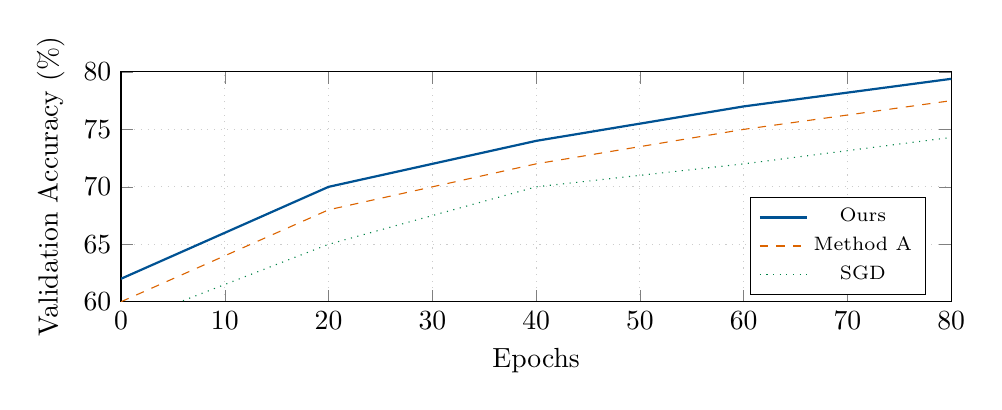
\begin{tikzpicture}
        \begin{axis}[
          width=\textwidth, height=4.5cm,
          xlabel={Epochs}, ylabel={Validation Accuracy (\%)},
          legend pos=south east,
          legend style={font=\scriptsize},
          grid=major, grid style={dotted,gray!40},
          xmin=0, xmax=80,
          ymin=60, ymax=80,
        ]
          \addplot[mlblue,thick] coordinates {(0,62)(20,70)(40,74)(60,77)(80,79.4)};
          \addplot[mlorange,dashed] coordinates {(0,60)(20,68)(40,72)(60,75)(80,77.5)};
          \addplot[mlgreen,dotted] coordinates {(0,58)(20,65)(40,70)(60,72)(80,74.3)};
          \legend{Ours, Method A, SGD}
        \end{axis}
      \end{tikzpicture}
    \end{column}
    \hfill
    \begin{column}{0.44\textwidth}
      \begin{block}{Component Analysis}
        \begin{itemize}
          \item w/o component A: $-1.8\%$
          \item w/o component B: $-0.9\%$
          \item Full model: \textbf{79.4\%}
        \end{itemize}
      \end{block}
    \end{column}
  \end{columns}
\end{frame}

% ── 5. CONCLUSIONS ────────────────────────────────────────────────────────────
\section{Conclusions}

\begin{frame}{Conclusions}
  \begin{block}{Contributions}
    \begin{enumerate}
      \item Novel method for [problem] with theoretical convergence guarantees
      \item State-of-the-art results on [benchmark], +1.4\% vs. best baseline
      \item Improved efficiency: 10 fewer epochs, 4h less training time
    \end{enumerate}
  \end{block}
  \vfill
  \begin{alertblock}{Limitations \& Future Work}
    \begin{itemize}
      \item Sensitivity to hyperparameter $\lambda$ -- adaptive tuning
      \item Extension to semi-supervised / self-supervised settings
    \end{itemize}
  \end{alertblock}
\end{frame}

% ── References ────────────────────────────────────────────────────────────────
\begin{frame}[allowframebreaks]{References}
  \bibliographystyle{plainnat}
  \bibliography{references}
\end{frame}

% ── Thank you ─────────────────────────────────────────────────────────────────
\begin{frame}
  \centering
  \vspace{1cm}
  {\Huge\bfseries\color{mlblue} Thank You!}\\[1em]
  {\large Questions \& Discussion}\\[2em]
  \begin{columns}[c]
    \begin{column}{0.45\textwidth}
      \centering
      \small
      \textbf{Code \& data:}\\
      \texttt{github.com/user/repo}
    \end{column}
    \begin{column}{0.45\textwidth}
      \centering
      \small
      \textbf{Contact:}\\
      \texttt{author@university.edu}
    \end{column}
  \end{columns}
\end{frame}

\end{document}
